\documentclass[12pt]{article}

\usepackage[a4paper,margin=1in]{geometry}
\usepackage{amsmath,amssymb}
\usepackage{tikz}
\usepackage{enumitem}
\usepackage{xcolor}

\setlength{\parindent}{0pt}
\setlength{\parskip}{0.75em}

\title{Lecture 11 Supplement: Exponential Waiting Times}
\author{MA4034 -- Time Series and Stochastic Processes}
\date{}

\begin{document}

\maketitle

\section{What Is a Waiting Time?}

Suppose events happen randomly over time according to a Poisson process.

Examples:
\begin{itemize}
    \item earthquakes in a region,
    \item phone calls arriving at a call center,
    \item customers arriving at a store,
    \item accidents happening on a road.
\end{itemize}

Let
\[
T_1=\text{time until the first event occurs}.
\]

If the Poisson process has rate \(\lambda\), then
\[
T_1\sim \operatorname{Exponential}(\lambda).
\]

The rate \(\lambda\) means:
\[
\lambda=\text{average number of events per unit time}.
\]

For example, if earthquakes occur at rate \(2\) per week, then
\[
\lambda=2.
\]

\section{The Main Formulas}

For
\[
T\sim \operatorname{Exponential}(\lambda),
\]
we have:

\[
f(t)=\lambda e^{-\lambda t}, \qquad t\geq 0.
\]

\[
F(t)=P(T\leq t)=1-e^{-\lambda t}.
\]

\[
P(T>t)=e^{-\lambda t}.
\]

\[
E[T]=\frac{1}{\lambda}.
\]

\section{Difference Between \(f(t)\) and \(F(t)\)}

This is very important.

\subsection*{\(f(t)\): Probability Density Function}

\[
f(t)=\lambda e^{-\lambda t}
\]
is called the \textbf{probability density function}.

It does \textbf{not} directly give the probability that \(T=t\).

For a continuous random variable,
\[
P(T=t)=0.
\]

So \(f(t)\) is not a probability by itself.

Instead, \(f(t)\) tells us how concentrated the probability is near time \(t\).

\begin{center}
\fbox{\parbox{0.85\textwidth}{
\[
f(t)=\text{height of the density curve at time }t.
\]
It is used to find probabilities over intervals.
}}
\end{center}

For example,
\[
P(1<T<3)=\int_1^3 f(t)\,dt.
\]

\subsection*{\(F(t)\): Cumulative Distribution Function}

\[
F(t)=P(T\leq t)
\]
is called the \textbf{cumulative distribution function}.

It gives an actual probability.

\begin{center}
\fbox{\parbox{0.85\textwidth}{
\[
F(t)=\text{probability that the first event happens by time }t.
\]
}}
\end{center}

For the exponential distribution,
\[
F(t)=1-e^{-\lambda t}.
\]

So if
\[
T\sim \operatorname{Exponential}(2),
\]
then
\[
F(1)=P(T\leq 1)=1-e^{-2}.
\]

This means:

\begin{center}
probability that the first event happens within 1 week.
\end{center}

\section{Why \(P(T>t)=e^{-\lambda t}\)}

Since
\[
F(t)=P(T\leq t),
\]
the opposite event is
\[
T>t.
\]

Therefore,
\[
P(T>t)=1-P(T\leq t).
\]

So
\[
P(T>t)=1-F(t).
\]

Using
\[
F(t)=1-e^{-\lambda t},
\]
we get
\[
P(T>t)=1-\left(1-e^{-\lambda t}\right).
\]

Thus,
\[
\boxed{P(T>t)=e^{-\lambda t}.}
\]

\section{Timeline Meaning}

\begin{center}
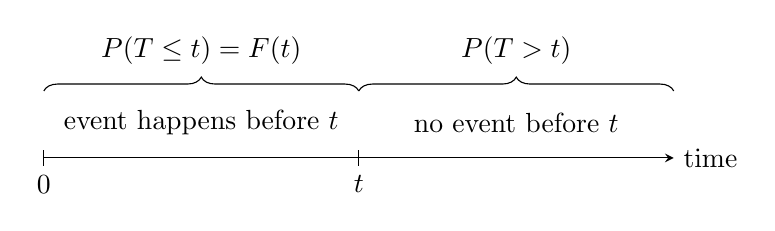
\begin{tikzpicture}[>=stealth, scale=1]
    \draw[->] (0,0) -- (8,0) node[right] {time};
    \draw (0,0.1) -- (0,-0.1) node[below] {0};
    \draw (4,0.1) -- (4,-0.1) node[below] {\(t\)};
    \node at (2,0.45) {event happens before \(t\)};
    \node at (6,0.45) {no event before \(t\)};
    \draw[decorate,decoration={brace,amplitude=5pt}] (0,0.85) -- (4,0.85)
    node[midway,above=6pt] {\(P(T\leq t)=F(t)\)};
    \draw[decorate,decoration={brace,amplitude=5pt}] (4,0.85) -- (8,0.85)
    node[midway,above=6pt] {\(P(T>t)\)};
\end{tikzpicture}
\end{center}

\[
F(t)=P(T\leq t)
\]
means the first event has already happened by time \(t\).

\[
P(T>t)
\]
means no event has happened yet by time \(t\).

\section{Connection With the Poisson Process}

Let \(N(t)\) be the number of events by time \(t\).

For a Poisson process with rate \(\lambda\),
\[
N(t)\sim \operatorname{Poisson}(\lambda t).
\]

The event
\[
T_1>t
\]
means the first event has not happened by time \(t\).

That is the same as saying:
\[
N(t)=0.
\]

Therefore,
\[
P(T_1>t)=P(N(t)=0).
\]

Since
\[
N(t)\sim \operatorname{Poisson}(\lambda t),
\]
we get
\[
P(N(t)=0)=e^{-\lambda t}\frac{(\lambda t)^0}{0!}.
\]

So
\[
P(N(t)=0)=e^{-\lambda t}.
\]

Hence,
\[
\boxed{P(T_1>t)=e^{-\lambda t}.}
\]

Then
\[
F(t)=P(T_1\leq t)=1-P(T_1>t).
\]

Therefore,
\[
\boxed{F(t)=1-e^{-\lambda t}.}
\]

\section{Expected Waiting Time}

For an exponential random variable,
\[
E[T]=\frac{1}{\lambda}.
\]

This means:

\begin{center}
\textit{larger rate means shorter average waiting time.}
\end{center}

For example:

\begin{itemize}
    \item If \(\lambda=2\) per week, then
    \[
    E[T]=\frac{1}{2}\text{ week}.
    \]
    On average, we wait half a week for the next event.

    \item If \(\lambda=10\) per hour, then
    \[
    E[T]=\frac{1}{10}\text{ hour}.
    \]
    Since \(1/10\) hour is 6 minutes, the average waiting time is 6 minutes.
\end{itemize}

\section{Simple Comparison Table}

\[
\begin{array}{c|c|c}
\text{Symbol} & \text{Meaning} & \text{Is it a probability?}\\
\hline
f(t) & \text{density at time }t & \text{No, not by itself}\\
F(t) & P(T\leq t) & \text{Yes}\\
P(T>t) & \text{probability waiting time exceeds }t & \text{Yes}\\
E[T] & \text{average waiting time} & \text{No, it is an average time}
\end{array}
\]

\section{Worked Example 1}

\textbf{Question.}
Earthquakes occur according to a Poisson process at rate \(2\) per week. Let \(T\) be the waiting time until the next earthquake.

\begin{enumerate}[label=(\alph*)]
    \item Find the density \(f(t)\).
    \item Find the probability that the next earthquake occurs within 1 week.
    \item Find the probability that we wait more than 1 week.
    \item Find the expected waiting time.
\end{enumerate}

\textbf{Answer.}

Here,
\[
\lambda=2.
\]

\textbf{(a)}
The density is
\[
f(t)=\lambda e^{-\lambda t}.
\]

So
\[
\boxed{f(t)=2e^{-2t}, \qquad t\geq 0.}
\]

\textbf{(b)}
Within 1 week means
\[
T\leq 1.
\]

So
\[
P(T\leq 1)=F(1).
\]

Using
\[
F(t)=1-e^{-2t},
\]
we get
\[
F(1)=1-e^{-2}.
\]

Therefore,
\[
\boxed{P(T\leq 1)=1-e^{-2}\approx 0.865.}
\]

\textbf{(c)}
More than 1 week means
\[
T>1.
\]

So
\[
P(T>1)=e^{-2(1)}=e^{-2}.
\]

Therefore,
\[
\boxed{P(T>1)=e^{-2}\approx 0.135.}
\]

\textbf{(d)}
The expected waiting time is
\[
E[T]=\frac{1}{\lambda}.
\]

Thus,
\[
\boxed{E[T]=\frac{1}{2}\text{ week}.}
\]

\section{Worked Example 2}

\textbf{Question.}
Customers arrive at a store according to a Poisson process with rate \(10\) per hour. Let \(T\) be the waiting time until the next customer arrives.

\begin{enumerate}[label=(\alph*)]
    \item Find \(P(T>0.5)\).
    \item Find \(P(T\leq 0.5)\).
    \item Interpret the answers.
\end{enumerate}

\textbf{Answer.}

Here,
\[
\lambda=10 \text{ per hour}.
\]

Also,
\[
0.5 \text{ hour}=30 \text{ minutes}.
\]

\textbf{(a)}
\[
P(T>0.5)=e^{-\lambda t}.
\]

So
\[
P(T>0.5)=e^{-10(0.5)}=e^{-5}.
\]

Therefore,
\[
\boxed{P(T>0.5)=e^{-5}\approx 0.0067.}
\]

\textbf{(b)}
\[
P(T\leq 0.5)=1-P(T>0.5).
\]

So
\[
P(T\leq 0.5)=1-e^{-5}.
\]

Therefore,
\[
\boxed{P(T\leq 0.5)=1-e^{-5}\approx 0.9933.}
\]

\textbf{(c)}
There is a very small chance of waiting more than 30 minutes, because the arrival rate is high.

\section{Worked Example 3}

\textbf{Question.}
Phone calls arrive at rate \(3\) per hour. What is the probability that no call arrives in the next 20 minutes?

\textbf{Answer.}

The rate is
\[
\lambda=3 \text{ per hour}.
\]

The time must also be in hours:
\[
20\text{ minutes}=\frac{20}{60}=\frac{1}{3}\text{ hour}.
\]

No call arrives in the next 20 minutes means
\[
T>\frac{1}{3}.
\]

So
\[
P\left(T>\frac{1}{3}\right)=e^{-3(1/3)}=e^{-1}.
\]

Therefore,
\[
\boxed{P(\text{no call in next 20 minutes})=e^{-1}\approx 0.368.}
\]

\section{Practice Questions}

\subsection*{Question 1}

Events occur according to a Poisson process with rate \(5\) per hour. Let \(T\) be the waiting time until the first event.

\begin{enumerate}[label=(\alph*)]
    \item Write \(f(t)\).
    \item Write \(F(t)\).
    \item Find \(P(T>0.2)\).
    \item Find \(E[T]\).
\end{enumerate}

\textbf{Answer.}

\[
\lambda=5.
\]

\textbf{(a)}
\[
\boxed{f(t)=5e^{-5t}, \qquad t\geq 0.}
\]

\textbf{(b)}
\[
\boxed{F(t)=1-e^{-5t}.}
\]

\textbf{(c)}
\[
P(T>0.2)=e^{-5(0.2)}=e^{-1}.
\]

So
\[
\boxed{P(T>0.2)=e^{-1}\approx 0.368.}
\]

\textbf{(d)}
\[
E[T]=\frac{1}{5}.
\]

So
\[
\boxed{E[T]=0.2\text{ hour}=12\text{ minutes}.}
\]

\subsection*{Question 2}

Buses arrive according to a Poisson process with rate \(4\) per hour. What is the probability that the next bus arrives within 15 minutes?

\textbf{Answer.}

The rate is
\[
\lambda=4 \text{ per hour}.
\]

Convert time:
\[
15\text{ minutes}=\frac{15}{60}=\frac{1}{4}\text{ hour}.
\]

Within 15 minutes means
\[
T\leq \frac{1}{4}.
\]

So
\[
P\left(T\leq \frac{1}{4}\right)=F\left(\frac{1}{4}\right).
\]

Using
\[
F(t)=1-e^{-4t},
\]
we get
\[
F\left(\frac{1}{4}\right)=1-e^{-4(1/4)}=1-e^{-1}.
\]

Therefore,
\[
\boxed{P(\text{next bus within 15 minutes})=1-e^{-1}\approx 0.632.}
\]

\subsection*{Question 3}

Accidents occur at rate \(2\) per week. What is the probability that the waiting time until the next accident is between 1 and 3 weeks?

\textbf{Answer.}

We want
\[
P(1<T<3).
\]

Using the CDF,
\[
P(1<T<3)=F(3)-F(1).
\]

Since
\[
F(t)=1-e^{-2t},
\]
we get
\[
F(3)=1-e^{-6}
\]
and
\[
F(1)=1-e^{-2}.
\]

Therefore,
\[
P(1<T<3)=(1-e^{-6})-(1-e^{-2}).
\]

So
\[
P(1<T<3)=e^{-2}-e^{-6}.
\]

Thus,
\[
\boxed{P(1<T<3)=e^{-2}-e^{-6}.}
\]

\subsection*{Question 4}

For an exponential waiting time, explain why \(f(2)\) is not the same as \(P(T=2)\).

\textbf{Answer.}

\(f(2)\) is the value of the density curve at \(t=2\). It is not a probability.

For a continuous random variable,
\[
P(T=2)=0.
\]

To get a probability, we need an interval, such as
\[
P(1<T<3)=\int_1^3 f(t)\,dt.
\]

So
\[
\boxed{f(2)\neq P(T=2).}
\]

\section{Summary}

\begin{itemize}
    \item \(f(t)\) is the density. It is the height of the curve, not a direct probability.
    \item \(F(t)=P(T\leq t)\) is the probability the first event happens by time \(t\).
    \item \(P(T>t)=e^{-\lambda t}\) is the probability we wait longer than \(t\).
    \item \(E[T]=1/\lambda\) is the average waiting time.
    \item Always match the unit of \(t\) with the unit of \(\lambda\).
\end{itemize}

\end{document}
